\documentclass{anstrans}
%%%%%%%%%%%%%%%%%%%%%%%%%%%%%%%%%%%
\title{Parallel Performance of the Time Dependent Transport Code TDKENO Applied to TREAT Simulations}
\author{Zander Mausolff,$^{*}$ Mark DeHart,$^{\dagger}$ Sedat Goluoglu $^{*}$}

\institute{
$^{*}$Nuclear Engineering Program, University of Florida
\\
529 Gale Lemerand Dr., Gainesville, FL, 32611
\and
$^{\dagger}$Nuclear Systems Design and Analysis Department Idaho National Laboratory 
\\
2525 North Freemont Street, Idaho Falls ID, 83415
}

\email{zanderm@ufl.edu $^{*}$} 


% Optional disclaimer: remove this command to hide
%\disclaimer{Notice: this manuscript is a work of fiction. Any resemblance to
%actual articles, living or dead, is purely coincidental.}

%%%% packages and definitions (optional)
\usepackage{graphicx} % allows inclusion of graphics
\usepackage{booktabs} % nice rules (thick lines) for tables
\usepackage{microtype} % improves typography for PDF

\newcommand{\SN}{S$_N$}
\renewcommand{\vec}[1]{\bm{#1}} %vector is bold italic
\newcommand{\vd}{\bm{\cdot}} % slightly bold vector dot
\newcommand{\grad}{\vec{\nabla}} % gradient
\newcommand{\ud}{\mathop{}\!\mathrm{d}} % upright derivative symbol

\begin{document}
%%%%%%%%%%%%%%%%%%%%%%%%%%%%%%%%%%%%%%%%%%%%%%%%%%%%%%%%%%%%%%%%%%%%%%%%%%%%%%%%
\section{Introduction}
Renewed interest in high fidelity simulation of excursion events has prompted the improvement of many codes that solve the time-dependent Boltzmann transport equation. Often these codes make approximations to the transport equation in order to achieve results in a reasonable amount of time.  One such method, the improved quasi-static (IQS), makes few approximations compared to adiabatic, diffusion, point kinetics, etc. The downside with this rigorous approach is computational time.  The code TDKENO employs the IQS method. To minimize the computational time associated with the flux shape calculation, a modified version of KENO-VI from Scale 6.2 is employed \cite{rearden2013overview}. This version of KENO runs in parallel across hundreds of nodes, resulting in drastically lower computational time.

The parallel capabilities of KENO allow TDKENO to simulate complex transient experiments with a large number of histories. These improvements are applied to the simulation of TREAT calibration experiments to aid in the restart and provide reference calculations for other codes. We present the improved computational overhead, memory usage, and accuracy for TDKENO in the case of simulating the entire TREAT core. 

%%%%%%%%%%%%%%%%%%%%%%%%%%%%%%%%%%%%%%%%%%%%%%%%%%%%%%%%%%%%%%%%%%%%%%%%%%%%%%%%
\section{Theory}
Solving the transport equation is non trivial when including the time dependence and explicit representation of delayed neutrons. Transient simulations resulting in the significant changes in the flux profile require rigorous methods to solve this "master equation" of reactor physics.  In TDKENO, the IQS method enables such simulations.  Utilizing the IQS method relies on the assumption that the total neutron flux can be factored into a shape and amplitude function \cite{Henry} \cite{Gehin}.  The amplitude function captures the time dependence and takes on physical significance by being cast into the form of the point kinetics equations,

\begin{equation}
    \frac{dP(t)}{dt} = \frac{\rho(t)-\bar{\beta}(t)}{\Lambda(t)} P(t) + \sum_{j=1}^{6} \lambda_jC_j(t) + \bar{Q}(t)
\end{equation}

where $P(t)$ is the amplitude function, $\rho$ is reactivity, $\bar{\beta}$ is the total delayed neutron fraction, $\Lambda$ is the generation time, $\lambda_j$ is the decay constant per neutron group $j$, $C_j$ is the density of delayed neutron precursors for group j, and $\bar{Q}$ is a source.  
 Reactivity, generation time, etc. (referred to as reactivity calculations) in TDKENO are found from their inner product definitions using a linearly interpolated flux shape and can be found in reference \cite{Bentley}.  Alternatively, these values may be computed during the Monte Carlo random walk but requires significant neutron histories to achieve low uncertainties \cite{Waddell}.  Whereas the shape function varies slowly in time and solves a modified version of the steady state transport equation.  The main modification here is an adjustment to the total cross section \cite{Bentley}\cite{Gehin}.  This allows for the flux distribution to vary in time and is why it becomes a necessary formulation to use in transient analysis.  In TDKENO the shape equation is solved via Monte Carlo, but in general the shape equation may be solved a variety of ways, such as a diffusion based code.  Reference \cite{Shayesteh} provides an excellent overview as to the rationale behind implementing Monte Carlo techniques for such calculations.  For the complete derivation of the IQS method employed in TDKENO, one can refer to reference \cite{Bentley}. 

Applying this factorization to the three-dimensional time-dependent transport equation with the explicit representation of delayed neutrons results in a set of coupled equations.  Equations for the flux shape, amplitude, and delayed neutron precursors are solved on several time scales through an iterative process with the relative sizes shown in Figure \ref{fig:time_scale}. 

\begin{figure}[h]
    \centering
    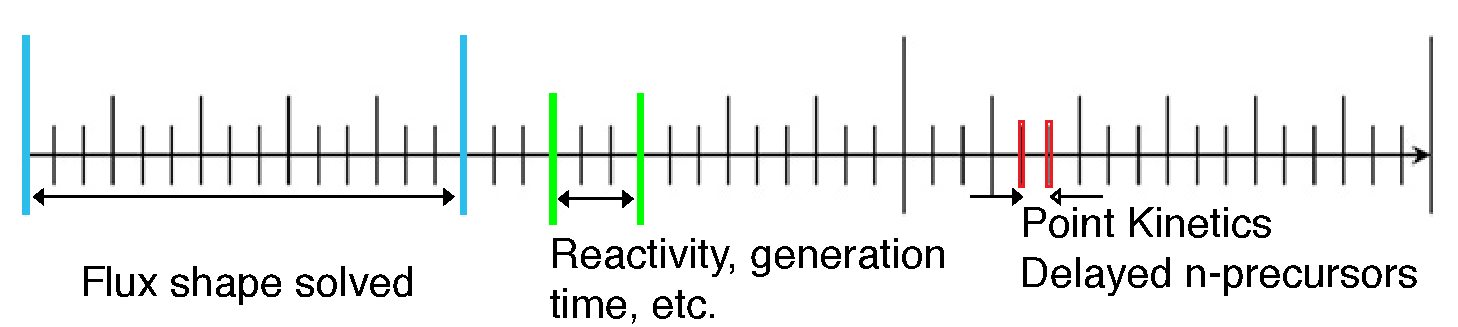
\includegraphics[width=8cm]{figures/time_scale.pdf}
    \caption{Time scale variation for IQS.}
    \label{fig:time_scale}
\end{figure}

The advantage of varying these time scales is computational overhead when compared to direct integration.  This comes from the flux shape being solved on a large time step. It is only done when the spatial distribution of neutrons changes significantly.  In between flux shapes, the corresponding differential equations are solved to capture the time dependent behaviour. The point kinetics equations are solved on the smallest time scale in between reactivity calculations.  In some IQS implementations, so called "Predictor Corrector" methods, conditions are evaluated to determine if the time step is too large to solve the flux shape \cite{Dulla}.  

%\begin{figure}[h]
%    \centering
%    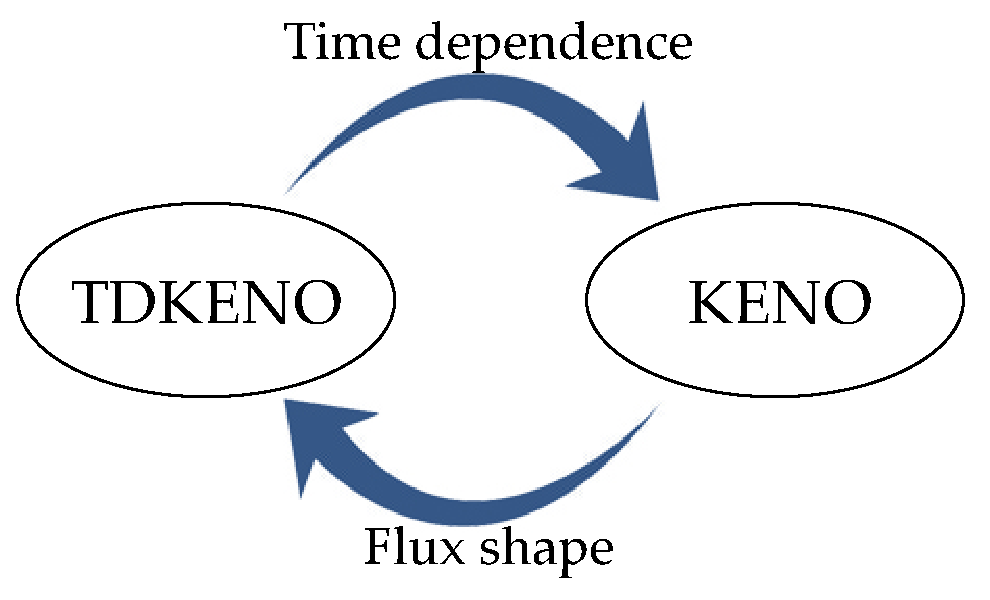
\includegraphics[width=7cm]{figures/tdkeno_flow.pdf}
%    \caption{Relationship between TDKENO and KENO.  TDKENO drives the time dependence, getting the %spatial neutron distribution from KENO.}
%    \label{fig:tdkeno_flow}
%\end{figure}

 In its current formulation, TDKENO does not do this but rather lets the user define when a flux shape should be calculated.  This gives flexibility and may allow for computational savings as transients experience a rapid change in neutron distribution that is generally known about \emph{a posteriori} and rapidly come to a steady state. Therefore, a new calculation of the flux shape is not required. However, since taking too large of a step is a possibility and may result in a less quality result, we are motivated to study the effects of varying the number of shape calculations.

%Equations look exceedingly pretty. Here is a 3-D, monoenergetic, steady-state
%transport equation with isotropic scattering and an isotropic extraneous source:
%\begin{subequations} \label{eqs:fullTransport}
%\begin{multline} \label{eq:fullTransportVol}
%  \vec{\Omega}\vd \grad \psi(\vec{x}, \vec{\Omega})
%  + \sigma(\vec{x}) \psi (\vec{x}, \vec{\Omega})
%\\ =
%  \frac{\sigma_s(\vec{x})}{4\pi} \int_{4\pi} \psi(\vec{x},\vec{\Omega}')
%  \ud\Omega' + \frac{q(\vec{x})}{4\pi}
%  \equiv \frac{1}{4\pi} Q(\vec{x}) \,,
%\end{multline}
%inside $\vec{x} \in V$, $\vec{\Omega} \in 4\pi$, with an incident boundary
%condition
%\begin{equation} \label{eq:fullTransportBndy}
%  \psi(\vec{x}, \vec{\Omega}) = \psi^b(\vec{x}, \vec{\Omega}) \,,
% \quad \vec{x} \in \partial V, \ \vec{\Omega} \vd \vec{n} < 0\,.
%\end{equation}
%\end{subequations}

%%%%%%%%%%%%%%%%%%%%%%%%%%%%%%%%%%%%%%%%%%%%%%%%%%%%%%%%%%%%%%%%%%%%%%%%%%%%%%%%
\section{Results and Analysis}
With the integration of the latest version of KENO from SCALE 6.2 we now have the ability to calculate the most intensive portion of the calculation in parallel \cite{rearden2013overview}.  Previously, for problems with complex geometry, the calculation of the shape may have taken several days to weeks to achieve adequate sampling and statistics.  By running TDKENO at the University of Florida's recently upgraded "HiperGator 2" supercomputer, we are able to run on hundreds of cores. As a result, these same calculations are only taking several hours. We apply these run time improvements to the particularly challenging problem of modeling the experiments done at the Transient Reactor Test Facility (TREAT). 

To evaluate the performance of TDKENO, one of the M8CAL experiments is simulated on varying numbers of nodes on the HiperGator while keeping all other parameters specific to the problem the same.  Each node has an Intel E5-2698 v3 (16 core, 2.3 GHz) with 4GB of RAM per node. Note that at present, only the flux shape is calculated in parallel.  The amplitude function and related quantities are solved in serial and are being investigated as to the potential improvements of calculating these quantities on graphic processing units (GPUs).  The M8CAL experiment being modeled is referred to in the documentation as the temperature limited transient \#2855 \cite{Robinson_Bauer_1994}.  This experiment was chosen as it has proven to be the most difficult to simulate compared to similar transients, referred to as \#2856 and \#2857 in references \cite{physor_mausolff} and \cite{kontogeorgakos2014treat}.  In previous modeling of these experiments, the experimental data compared to was thought to have inconsistencies with the values reported in the write up \cite{physor_mausolff}.  However, upon further inspection, the data that corresponds to the M8CAL reported values has been found, digitized, and compared to the results shown here.

%%%%%%%%%%%%%%%%%%%%%%%%%%%%%%%%%%%%%%%%%%%%%%%%%%%%%%%%%%%%%%%%%%%%%%%%%%%%%%%%
\subsection{Computational Improvements}

The computational improvements are highlighted in TDKENO by comparing the same problem run on an increasing number of cores.  In this case, the KENO calculations were run with 10000 particles per generation with a total of 2500 generations. A total of 14 flux shapes were calculated with KENO at times primarily centered around the first few seconds.  We have chosen these numbers as they appear to give almost identical results to simulations run with many more histories as seen in Figure \ref{compare_hist}.  Simulations run with additional histories do result in less statistical uncertainties in values such as fluxes, keff, etc.  These are of less interest in this paper.  

\begin{figure}[h]
    \centering
    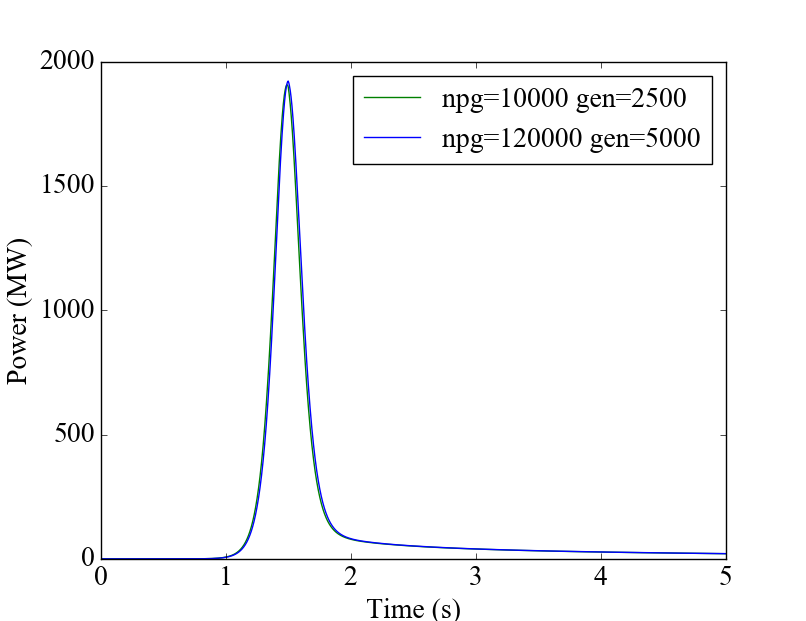
\includegraphics[width=9cm]{figures/comp_npg2855.png}
    \caption{The calculated power vs. time is compared between TDKENO simulation of TREAT transient \#2855 with differing numbers of histories. }
\end{figure}

The model of the TREAT core used contains approximately 4000 regions with 21 materials using KENO-VI generalized geometry.  The TREAT core is unique in its ability to safely have simulate large reactivity insertions.  It accomplishes this with a core composed of 93.1\% $UO_2$ embedded in a graphite matrix, with a ratio of $UO_2$ to graphite of approximately 1:10000.  Details about the TREAT core may be found in \cite{bess2015baseline}.  A variety of control rods are available and the transient shown in this paper is induced by the rapid withdrawal of transient rods over 0.13 seconds. 

Below we show the affect of increasing the number of cores the problem is run on.  The relatively low number of histories results in poor scaling to large number of cores due to increased communication time and less work done by each core.  The communication time is compounded because the flux shape calculation is done in parallel with the results gathered on the master.  This master processor then computes the point kinetics values in serial.  Nevertheless the performance is drastically improved when compared to serial even with a modest amount of processors (for high performance computing standards).  
\begin{table}[h]
    \centering
    \begin{tabular}{c|c}
                    Total Cores  & Elapsed Time (minutes) \\
                    \hline 
                    1                  &   12,347            \\
                    16                 &   1,560             \\
                    32                 &   1,619              \\
                    48                 &   1,356              \\
                    64                 &   1,051             \\
                 %   80                 &                \\  
                    96                 &   917             \\
                    160                &   810             \\
                    \hline
    \end{tabular}
    \caption{Variation of the number of cores run for the simulation of \#2855. Elapsed time generated from the SLURM submission system \cite{yoo2003slurm}. }
    \label{tab:parallel}
\end{table}
Improvements could be made to further optimize the inputs by judiciously choosing the number of particles such that an integer amount is calculated on a single core.  Such methods may improve load balancing and communication time.  However, this is something a user should not be thinking about and these results are more indicative of "real world" behaviour.

%The poor parallel efficiency is further evidenced when inspecting the efficiency as measured by %KENO for a single flux shape.  

\begin{figure}[h]
    \centering
    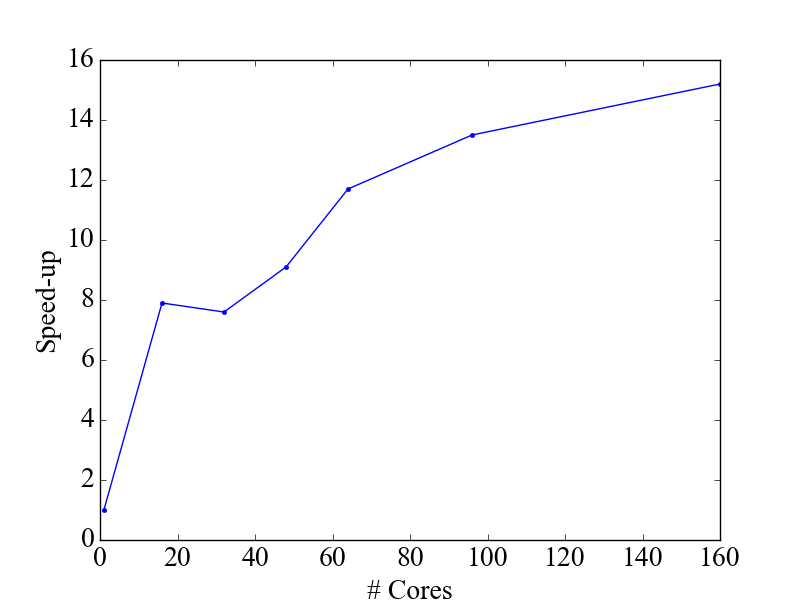
\includegraphics[width=9cm]{figures/speedup.png}
    \caption{Speed-up measured relative to the execution time on a single core.}
    \label{fig:speedup}
\end{figure}

%%%%%%%%%%%%%%%%%%%%%%%%%%%%%%%%%%%%%%%%%%%%%%%%%%%%%%%%%%%%%%%%%%%%%%%%%%%%%%%%
%\subsection{Flux Shape Variation}
%M8CAL 2855 only?
%
%\begin{table}[h]
%    \centering
%    \begin{tabular}{c|c|c}
%         & TDKENO-K5 & TDKENO-K6 \\
%        Generations &  10000 & 10000 \\
%        Particles   &  10000 & 10000 \\
%        Skipped     &  500   & 500  \\
%    \end{tabular}
%    \caption{Caption}
%    \label{tab:my_label}
%\end{table}

\subsection{Point Kinetics Variation}
As mentioned, the IQS methodology  splits the transport equation into several coupled equations solved on three time scales.  These definitions are readily available and can be found in reference \cite{Bentley}.  Each of the scales may be chosen by the user providing an integer number.  This number indicates the amount of calculations done between flux shapes.  For example, one can specify to do 10 point kinetics solves per reactivity calculation and 20 reactivity calculations, for a total of 200 calculations in-between flux shapes.  As stated previously, these equations are formulated to contain the time dependence and must be solved when the system undergoes significant changes (e.g. reactivity insertion).  In its current state there are no methods to verify if too few calculations are chosen. To ensure time dependent behaviour is not missed, we have been performing a large number of calculations between flux shapes.  These do not take too long to compute in general but we are motivated to mitigate this number for several reasons.  One, examining increasingly complex problems results in models with thousands of regions and the number of regions is directly proportional to the calculation time.  Second, with the parallel integration the calculation time of the flux shape and point kinetics calculations become next portion of the code necessary to speed up.

   Several simulations were performed with the number of times reactivity calculations increased each time while the point kinetics equations are solved at same frequency.  The quantity of most interest in these transient experiments is the total energy deposited in the core, thus is a number we would like to simulate accurately.  Additionally, experimental values for the yield and power as a function of time are reported for this experiment.  In previous  papers, the experimentally values were not transcribed properly and were slightly off \cite{physor_mausolff}.  What is shown here aligns with the values reported in the original experimental report \cite{Robinson_Bauer_1994}.  Both experimental and all calculated values for the yield as function of time are found in Figure \ref{fig:ptkinvar}.  The first 10-90 reactivity calculations all use 10 point kinetics solves.  The 100 line in Figure \ref{fig:ptkinvar} is the typical number we have been using and used 100 point kinetics solves.  The 500 line is an extreme case, with 500 reactivity and 500 point kinetics solves. Clearly this doesn't improve the solution at all.
   
   From about 10 to 50 reactivity calculations, there is an obvious deviation that gives a final yield very far off from the experimental value.  After 60 reactivity calculations, further increases do not appear to give a different solution.  It appears one could get away with this many calculations and not suffer a loss of accuracy.

\begin{figure}[h]
    \centering
    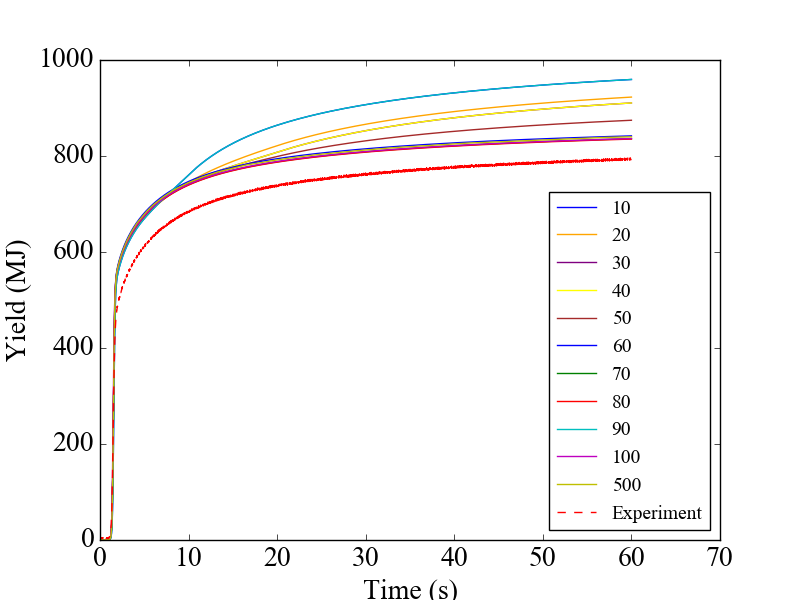
\includegraphics[width = 9 cm]{figures/ptkinvar.png}
    \caption{Varying the number of reactivity calculations between macro time steps.}
    \label{fig:ptkinvar}
\end{figure}

The goal behind minimizing the number of calculations in-between flux shape updates is computational savings.  To evaluate this we look at the total CPU time spent in-between flux shapes for the entire simulation.  This was done with a utility in TDKENO that measures the wall clock time between flux shapes and finds a total CPU time. We plot the calculation time for reactivity calculations 10-90 in Figure \ref{fig:ptkin_time}.  

\begin{figure}[h]
    \centering
    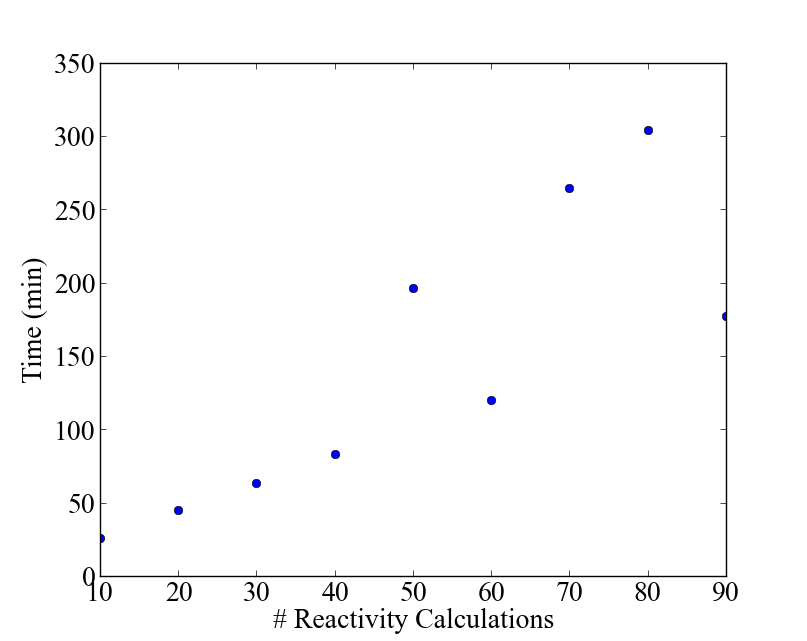
\includegraphics[width=9cm]{figures/ptkin_time_var.png}
    \caption{Total CPU time plotted against the number of reactivity calculations. }
    \label{fig:ptkin_time}
\end{figure}

There appears to be a linear trend as the number of reactivity calculations increases.  However, there are 3 outliers.  There is reason to believe these 3 runs are not representative of the general behaviour of TDKENO. The deviations may be attributed to running them on the HiperGator 2. These runs requested 5 nodes with 8 cores per node, which is only half the cores available on the node.  It is possible that during the runs, another program may have been using the other 8 cores and oversubscribed the node memory.  Other anomalies were present in runs performed with the same parameters, with the only difference being the number of cores run on.  For instance, looking at the CPU time for reactivity calculations on the runs shown in Figure \ref{fig:speedup} showed consistent behaviour, except for the run performed on a total of 80 cores as seen in Figure \ref{fig:ptkin_same_time}. These simulations were performed during the first month of operation of the HiperGator 2 and the system may not been optimized.  In general inspecting Figure \ref{fig:ptkin_same_time} shows the typical time spent calculating the reactivity/point kinetics is approximately 300 minutes.  Comparing that to the minimum number required to get the same answer (60 reactivity calculations as per Figure \ref{fig:ptkin_time}) about 180 minutes could be saved.  

It is clear that minimizing the number of reactivity calculations improves computational time without sacrificing the final solution quality.  This motivates future work in several ways.  This time is not insignificant and can be further improved with parallelization on CPUs or GPUS.  Additionally, that determining criteria when the solution is converged is desirable to prevent unnecessary computational time.   

\begin{figure}[h]
    \centering
    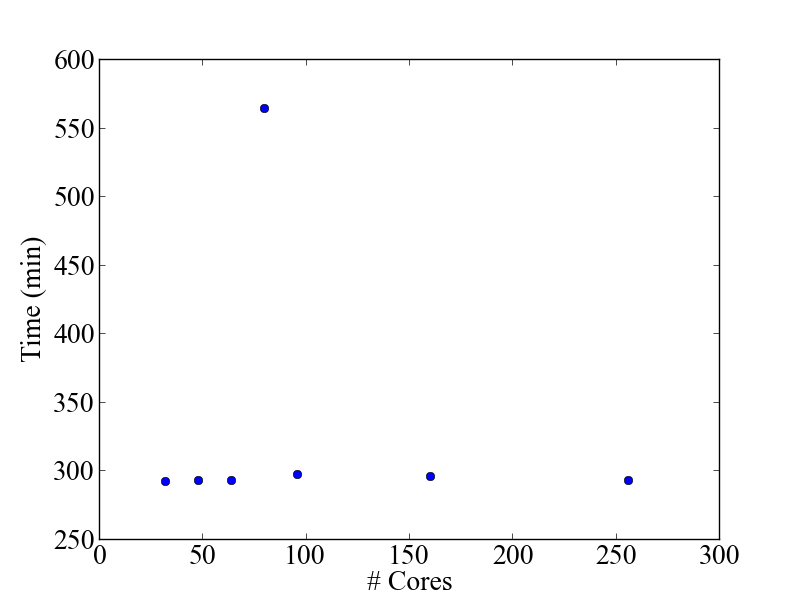
\includegraphics[width=9cm]{figures/comp_time_same-ptkin.png}
    \caption{Comparison of total CPU time for reactivity/point kinetics calculations while the number of cores each simulation is run on is varied.}
    \label{fig:ptkin_same_time}
\end{figure}

%%%%%%%%%%%%%%%%%%%%%%%%%%%%%%%%%%%%%%%%%%%%%%%%%%%%%%%%%%%%%%%%%%%%%%%%%%%%%%%%
\section{Conclusions}
The integration of a parallel flux shape solver has resulted in a transient analysis tool that is up to 15 times faster than previous implementations on a single core.  It is not practical to run many simulations on increasingly complex problems without waiting months for a result. Such nuanced behaviour such as the variation of reactivity calculations during a TDKENO run may now be studied in detail to further improve the method.  It has been shown for difficult problems like TREAT simulations, the deterministic portions of the code take significant CPU time and are ripe for parallelization implementations. Future work will be to determine convergence criteria for the reactivity and point kinetics equations and have these done in parallel, likely on GPUs. 

%%%%%%%%%%%%%%%%%%%%%%%%%%%%%%%%%%%%%%%%%%%%%%%%%%%%%%%%%%%%%%%%%%%%%%%%%%%%%%%%

%%%%%%%%%%%%%%%%%%%%%%%%%%%%%%%%%%%%%%%%%%%%%%%%%%%%%%%%%%%%%%%%%%%%%%%%%%%%%%%%
\section{Acknowledgments}
This material is based upon work supported by the Idaho National Laboratory.

%%%%%%%%%%%%%%%%%%%%%%%%%%%%%%%%%%%%%%%%%%%%%%%%%%%%%%%%%%%%%%%%%%%%%%%%%%%%%%%%
\bibliographystyle{ans}
\bibliography{bibliography}

\end{document}

